\chapterOrPart{Useful commands}\label{ch:usefulcommands}
This chapter contains an alphabetic list of some useful commands. All the commands that are mentioned here are included in the style file \verb|styles/myCommands|.

\section{Basic commands in \LaTeX}
There are several good sources to learn about commands in \LaTeX. See for instance the list below
\begin{itemize}
    \item \href{https://www.ntg.nl/doc/biemesderfer/ltxcrib.pdf}{\LaTeX\ command summary}
    \item \href{https://wch.github.io/latexsheet/}{\LaTeX\ cheat sheet}
    \item \href{https://en.wikibooks.org/wiki/LaTeX/Command_Glossary}{Wikibook: \LaTeX\ command glossary} 
\end{itemize}

Below we will mention some commands that might be of interest for you.

\section{\textbackslash chapterOrPart}
This command is defined in \texttt{styles/myCommands.sty}. It starts a new chapter when compiled with the class \pkg{memoir} to make a report or thesis. But it will start a new part, instead of a new chapter, when compiled with the class \pkg{beamer} to make slides. The reason being that the concept of a chapter does not exist in a presentation made with \pkg{beamer}. The \cs{ChapterOrPart} command also executes a \cs{mode*} command so that content outside frame environments is ignored when compiling with \pkg{beamer}, see also \cref{sec:mode}.

\section{\textbackslash def}
This command is typically used to define constants that can be accessed and employed across your entire document. The constants can be numerical or text strings. The syntax is\\ \verb|\def\commandname{replacement}| where \cs{commandname} is the name of the command you want to define, and \texttt{replacement} is the value or text that will be substituted when the command is used. In this template, you can find several examples of the use of \cs{def}.

For an example of a definition of a numerical constant, see the command \verb|\def\arcr{0.8cm}| in the source code of \cref{fig:freebody}. It assigns the value of 0.8~cm to \verb|\arcr| and is then used as the radius of the arc to indicate angles in the free body diagram. Feel free to adapt this value and observe the effect on the free body diagram after a recompile.

For defining of text strings, inspect the files \texttt{extra/titleInfoVUB} and \texttt{extra/titleInfoULB}, where you will find definitions of text strings that are used to compose the VUB and ULB title pages. Other examples can be found in the file \texttt{extra/nomenclature}, where section names for the nomenclature are defined, depending on the document language. The document language is part of the options of the command \texttt{\textbackslash documentclass[\dots]} at the first line of the main file. For your info: the current language of a document can be displayed with the command \verb|\languagename|. In this document, it is currently set to: \texttt{\languagename}\footnote{Reminder: names of language options are not capitalized in \LaTeX.}.

Warning: the command \cs{def} does not check if a command name already exists, so it does not prevent accidental redefinition of existing commands. So exercise caution to prevent unintentional overwriting of existing commands. If you want error checking, use \cs{newcommand} instead, as explained in \cref{sec:newcommand}.

\section{\textbackslash definecolor}
You can define your own colours. For instance:

\verb|\definecolor{VUBorange}{cmyk}{0.00, 0.78, 1.00, 0.00}|

defines the colour VUBorange. This colour can now be used in your document, as is done on the title page. For instance, the command 

\verb|\textcolor{VUBorange}{This text is written in VUB orange}|

will produce: \textcolor{VUBorange}{This text is in VUB orange}.

\section{\textbackslash ensuremath}
The command \cs{ensuremath} ensures that its argument is enclosed in math mode, regardless of whether the surrounding text is in math mode or regular text mode. It is typically used inside \cs{newcommand}. For instance, the command \verb|$\psat$| will produce $\psat$ but the command without the dollar-signs \cs{psat} will produce exactly the same result. This is because the command \cs{ensuremath} is used inside the definition of \cs{psat} (you can verify this in the style file \verb|styles/myCommands|). It will force a switch to math mode, if not yet in math mode. This is very convenient because you are no longer obliged to explicitly activate math mode with the \$-signs, every time you use such a command when writing.

\section{\textbackslash hideExplanations}
The command \cs{hideExplanations} will hide the explanations in blue at the beginning of chapters. You will find this command in the preamble of \texttt{mainReport} where is currently command out so the explanations are visible. 

\section{\textbackslash include}
The command \cs{include\{\meta{filename}\}} is used to include chapters. It will process all the floats (figures and tables) from the previous chapter, cause a page break so that the next chapter can start on a new page and import the content from the file named \meta{filename} into the document body. It will also start a new auxiliary file in the background to keep track of the locations of figures, tables and equations within the chapter for proper cross-referencing. It is not possible to nest \cs{include} commands.

\section{\textbackslash includeonly}
This command is used to reduce the compilation time of your Overleaf project. There are two ways to reduce compilation time:
\begin{enumerate}
    \item Reduce the amount of content in the document part. This can be achieved by disabling \cs{include}\marg{path/filename} commands. Just put a \%-sign at the beginning of each line that you want to exclude. For instance: 
    \verb|%\chapterOrPart{Introduction}\label{ch:introduction}

% \begin{explanation}
%     A thesis typically contains an introduction. A possible structure is provided below. 
%     \begin{itemize}
%         \item Context: situate your work within a broader background and explain the relevance of the problem your work addresses
%         \item Topic: define the topic and scope of your work
%         \item Research question: list the research question(s) that your work aims to answer; a master thesis and a PhD must have research questions
%         \item Objectives: list the objectives of your work
%         \item Thesis structure: briefly describe the thesis structure
%     \end{itemize}
% \end{explanation}

\section{Context}

Residential energy demand is becoming a more difficult object to model because two transitions are occurring at the same time. Climate change alters the weather conditions that drive space-heating and cooling pressure, while residential technologies such as heat pumps, photovoltaic (PV) systems and electric vehicles (EVs) change the carriers, timing and coincidence of household electricity demand. For Belgium this interaction is especially relevant because the residential stock remains strongly heating-dominated and still relies substantially on fossil heating carriers, while electrified end uses are expected to become more prominent \cite{eurostat_disaggregated_nodate,JRC2022HeatPumpBelgium,Statbel2025EV}.

The technical challenge is not only to estimate annual energy consumption. Future residential demand also depends on the temporal structure of demand, the conversion of useful heat into gas or electricity, PV self-consumption and export, EV charging, and the diversity of household behaviour. Bottom-up modelling is useful in this setting because it can represent dwellings, end uses, weather forcing, technology assumptions and stochastic household differences explicitly rather than treating residential demand as a single aggregate time series \cite{Richardson2010CRESTElectricity,McKenna2015}. Climate-impact modelling adds a further requirement: weather and climate scenarios must be propagated through the demand model in a way that keeps the difference between climate forcing, technology assumptions and stochastic variation visible \cite{IPCC2021,DeWilde2014,Jacob2014EuroCordex}.

\section{Problem Statement}

Many residential demand assessments treat climate sensitivity, technology uptake and behavioural diversity as separate modelling problems. This is limiting for an electrifying residential system. A warmer climate can reduce useful space-heating demand, but electrified heating can simultaneously increase winter electricity peaks. PV can reduce net grid import at some hours, but its value depends on temporal overlap with household demand. EV charging can add annual electricity demand, but its impact on grid stress depends on when charging occurs and how coincident it is across households. A model that reports only annual energy can therefore miss the system-relevant part of the transition.

The knowledge gap addressed in this thesis is the combined treatment of climate forcing and residential technology-stock assumptions in a traceable Belgian bottom-up demand model. The model must distinguish useful thermal demand from final energy carriers, preserve household-to-household variation, report grid import and export at the active timestep, and state clearly which claims are supported by validation evidence. The aim is not to produce a calibrated national forecast of Belgian residential demand, but to build and evaluate a reproducible scenario framework that can show how climate and technology assumptions shape residential final energy, carrier use and peak electricity load under stated conditions.

\newpage
\section{Research Question}

The central research question is:

\begin{quote}\itshape
How do climate forcing and residential technology-stock assumptions interact to shape future Belgian household final energy demand, carrier use, and peak electricity load?
\end{quote}

This question is operationalised through four supporting questions. First, the thesis asks how climate forcing affects residential space-heating demand and overheating indicators under a frozen technology stock. Second, it asks how electrification, PV and EV technology cases change final-energy carrier use and grid import/export profiles. Third, it asks how large stochastic household-to-household variability is relative to climate- and technology-driven differences. Fourth, it asks to what extent the model can reproduce Belgian residential demand patterns against macro, synthetic, smart-meter, PV and EV validation references.

\section{Research Objective}

The objective is to develop and evaluate a stochastic, physics-informed bottom-up model for Belgian residential energy demand under climate and technology uncertainty. The model combines Belgian dwelling and technology-stock assumptions, occupancy-conditioned stochastic demand generation, a reduced-order thermal balance, heat-pump and carrier-conversion logic, PV and EV modules, and a scenario-tree layer that records provenance for each executed scenario leaf. The output of interest is not one forecast year, but a set of conditional comparisons across climate windows, RCP pathways, technology cases and stochastic realisations.

The scope is deliberately bounded. The model represents residential demand at the dwelling-meter boundary and reports final energy, carrier use, PV generation, grid import/export, peak import, heating and cooling pressure indicators, and selected economic and emissions post-processing outputs. It does not model distribution-network power flow, endogenous technology adoption, active cooling final electricity demand, embodied emissions, or a multi-model climate ensemble. Future climate results are therefore interpreted as conditional scenario results under the configured CORDEX chain rather than as probabilistic forecasts.

\section{Thesis Structure}

\Cref{ch:literature} reviews residential energy demand, bottom-up modelling, uncertainty, climate forcing and validation approaches. \Cref{ch:materialsmethods} defines the model scope, input data, scenario-tree system, demand model, technology modules, output ledger and validation strategy. \Cref{ch:results} reports the executed model configurations, validation evidence and climate-scenario results. \Cref{ch:discussion} interprets the results for adaptation, electrification, limitations and future work. \Cref{ch:conclusions} closes the thesis by answering the research question directly from the results.

\mode<all> % do not remove




% % \begin{explanation}
% % It is recommended to use action verbs to formulate objectives. It will make them actionable and easier to assess for progress. Examples of action verbs are: to analyze, assess, build, construct, create, demonstrate, design, develop, evaluate, enhance, implement, improve, increase, investigate, measure, optimize, produce, reduce, test, validate.

% % Try to formulate \href{https://en.wikipedia.org/wiki/SMART_criteria}{SMART} objectives that are specific, measurable, achievable, relevant, and time-bound. This approach will help make your objectives clearer, easier to track, realistic, aligned with your research question and defined within a specific time frame for completion.



% % Example of a SMART objective: "To measure the PM emissions from a multiheat wood pellet boiler with an ELPI+ during 24 hours of continuous operation at 100\% load in December 2025."

% % The non-SMART version: "Study boiler emissions"
% % \end{explanation}

% \section{Thesis structure} 
\mode<all> % do not remove
| 
    will no longer compile the \verb|introduction| file. As a result:
        \begin{itemize}
            \item The content of \verb|introduction| will no longer be known to \LaTeX, and thus will no longer show up in the output PDF
            \item The content of \verb|introduction| will no longer show up in the table of contents
            \item Labels in \verb|introduction| will no longer be known to \LaTeX, so cross-references to these labels, from anywhere in your document, will result in broken links, indicated by a double question mark: ??
        \end{itemize}
    \item Use the command \cs{includeonly}\marg{path/filename} in the \textit{preamble}. But beware, you must proceed as follows:
    \begin{enumerate}
        \item First compile your entire project. You can achieve this by putting a \%-sign in front of the \cs{includeonly} command in the \textit{preamble}. This will allow \LaTeX\ to detect the entire document structure (chapters, sections, labels, \dots) in all the included files.
        \item After successful compilation, you can now restrict compilation to the file you are currently working in. Let's assume it is the \verb|introduction| file. In that case, you add the command \verb|\includeonly{chapters/introduction}| to your \textit{preamble}\footnote{Do not add the \cs{includeonly} command to the document part, it does not belong there and will cause an error.}. As a result:
      \begin{itemize}
            \item Only the content of \verb|introduction| will be recompiled by \LaTeX. The other included files are not recompiled. This will speed up compilation! The content of all the other compiled files is however still known to \LaTeX\ from the previous full compile. 
            \item Only the content of \verb|introduction| will show up in the output PDF.
            \item The content of all included files will show up in the table of contents, because \LaTeX\ remembers the document structure from the first entire compile.
            \item All the labels in all compiled files are known to \LaTeX, so cross-references to such labels, from anywhere in your document, will work.
        \end{itemize}
    \end{enumerate}
\end{enumerate}

\section{\textbackslash includegraphics}
The \cs{includegraphics} command is used to include images or other types of graphics in your document. Often included file types are PDF, PNG and JPG. PDF is preferred over PNG or JPG because it is a vector format and thus it retains its image quality on all zoom levels. 
The general form of the command is \cs{includegraphics}\oarg{options}\marg{filename}. Often used options are listed in \cref{tab:includegraphicsoptions}. When more than one option is specified, they will be processed in the order they are specified, so from left to right. This is important when combining sizing and rotating of an image.

\begin{table}\centering
    \caption{Often used options for \cs{includegraphics}}
    \renewcommand{\arraystretch}{1.3} % Default value: 1
    \begin{tabular}{lp{7.5cm}}
    \toprule
    option example                                   & explanation \\[+1ex]
    \verb|width=0.8\textwidth|                       & set image width to 80\% of the textwidth, height is scaled proportionally\\
    \verb|height=0.7\textheight|                     & set image height to 70\% of the textheight, width is scaled proportionally\\
    \verb|keepaspectratio|                           &  ensures that the aspect ratio of the image is maintained when both width and height are specified\\
    \verb|scale=0.6|                                 & scale image to 60\% of size\\
    \verb|angle=30|                                  & rotate image \qty{30}{\degree} counterclockwise\\
    \verb|frame|                                     & add frame around image\\
    \verb|trim={1cm 2cm 3cm 4cm}|                    & hide parts of image: 1 cm from left, 2 cm from bottom, 3 cm from right, 4 cm from top\\
     \verb|clip|                                     & remove parts of image that were hidden via trim\\
    \bottomrule
    \end{tabular}\label{tab:includegraphicsoptions}
\end{table}

The command is provided by the package \pkg{graphicx}, a widely used package in LaTeX for handling graphics. More info at \href{https://ctan.org/pkg/graphicx?lang=EN}{CTAN: package graphicx}.

\section{\textbackslash includesvg}
The \cs{includesvg} command is used to include Scalable Vector Graphics (SVG) files in your document. SVG is a widely used vector image format that allows for high-quality images at any scale without loss of resolution.

The general form of the command is \cs{includesvg}\oarg{options}\marg{filename}. It is provided by the package \pkg{svg}. More info at \href{https://ctan.org/pkg/svg?lang=EN}{CTAN: package svg}.

\section{\textbackslash input}
The \cs{input}\marg{filename} command is used to insert the contents of another file named \meta{filename} into the document body. It's equivalent to typing all the content from the file named \meta{filename} into the target file at the location of the \cs{input\{\meta{filename}\}} command. It is used to break up your project into smaller, more manageable parts. It will not start on a new page. It is possible to nest \cs{input} commands.

\section{\textbackslash intertext}
The command \cs{intertext} is useful to write lines of text between equations. It is applied in the \verb|align| environment. You can then use one single \verb|align| environment, instead of a series of separate \verb|equation| environments. Inspect the source code in the example below. This approach is also very well suited for writing equations on slides.
\begin{frame}{Text can be placed between aligned equations with \cs{intertext}}
    \begin{align}
        \intertext{For an adiabatic CV, the entropy balance is} 
        &\dod{S_\CV}{t}=\sum_\up{in}\mdot_i\cdot s_i-\sum_\up{out}\mdot_j\cdot s_j+\dot{S}_\up{gen}\\
        \intertext{for a closed CV with $k$ heat flows, it takes the following form}
        &\dod{S_\CV}{t}=\sum\frac{\qdot_k}{T_k}+\dot{S}_\up{gen}\\
        \intertext{and for an isolated CV it reduces to}
        &\dod{S_\CV}{t}=\dot{S}_\up{gen}\geq 0\qquad\text{and thus $S$ reaches a maximum at equilibrium.}\label{eq:Smax}
    \end{align} 
\end{frame}

\section{\textbackslash mathrm}\label{sec:mathrm}
The command \cs{mathrm} is used to write upright symbols in mathematical expressions, such as for example the Reynolds number in \cref{eq:mathrm}. See also the shorter command \cs{up} with the same effect, discussed in \cref{sec:up}.
\begin{equation}\label{eq:mathrm}
    \mathrm{Re}=\frac{\vel\cdot L}{\viscokin}
    % \vel       = symbol for velocity defined in \styles\myCommands
    % \viscokin = symbol for kin. viscosity defined in \styles\myCommands
\end{equation}

\section{\textbackslash mode}\label{sec:mode}
Read this section if you want to understand how one source file can be used for different outputs. The \cs{mode} command is used to control the inclusion of content based on the mode in which the document is being compiled. This is useful for source files that are used to serve multiple purposes, for instance to generate slides and to make a report/thesis.

The \pkg{beamer} class supports seven modes, as shown in \cref{fig:modes}, each designed for different output formats. As you likely already know, this template utilizes two classes. When you compile with class \pkg{beamer} to create slides, the <presentation> mode is active. Conversely, when you compile with class \pkg{memoir}  to produce a report or thesis, the <article> mode is active. The name of the <article> mode is somewhat misleading, because it is not only active when you compile a project with the \pkg{article} class. It is active for all output types that are not presentations. So when you compile with classes like \pkg{book}, \pkg{article}, \pkg{report}, or \pkg{memoir}, the <article> mode is active.

By using \cs{mode<presentation>}\marg{content} or \cs{mode<article>}\marg{content}, you can specify content that will only be processed when the respective mode is active. This is for instance used in \texttt{styles/myPageSetup.sty} to perform a separate page setup for the slides and for the report/thesis.

\begin{figure}\centering
    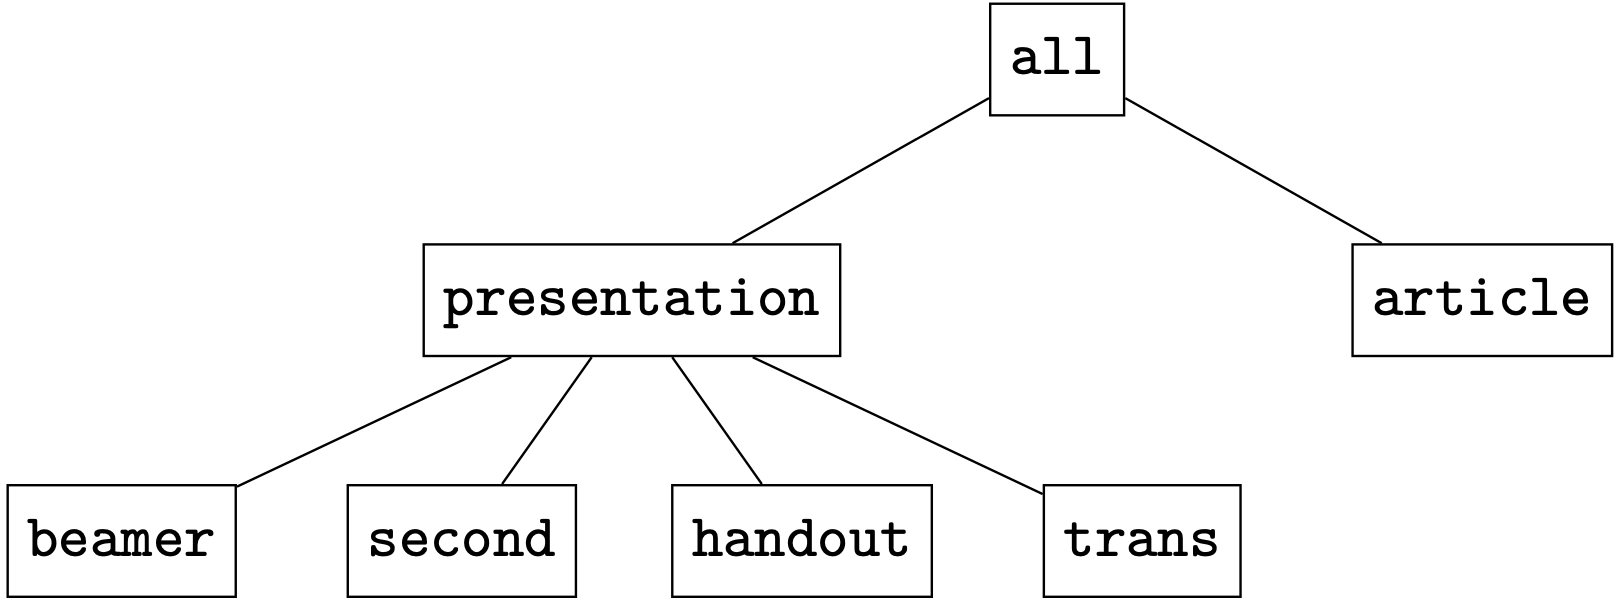
\includegraphics[width=0.6\textwidth]{figs/modes}
    \caption{The seven modes in \pkg{beamer} (\href{https://nl.mirrors.cicku.me/ctan/macros/latex/contrib/beamer/doc/beameruserguide.pdf}{beamer manual, p. 205})}
    \label{fig:modes}
\end{figure}

There are two additional commands related to modes that are frequently used throughout this template. The first one is the \cs{mode*} command which is particularly useful when compiling with the \pkg{beamer} class, as it ensures that the compiler ignores all content that is not within frame environments. This command is typically placed at the beginning of tex file, and in this template, it is incorporated into the \cs{chapterOrPart} command, which is defined in \texttt{styles/myCommands.sty}. The second command is \cs{mode<all>} which instructs the compiler to process all content, and it is generally written at the end of tex file. Without \cs{mode<all>} at the end of a tex file, the subsequent \cs{chapterOrPart} command in the next tex file would be ignored, as it would fall outside a frame environment.

\section{\textbackslash newcommand}\label{sec:newcommand}
With the command \cs{newcommand} you can define your own commands. That can be useful to simplify repetitive and/or complex formatting. See the \href{https://www.overleaf.com/learn/latex/Commands#Defining_a_new_command}{Overleaf documentation on newcommand} for more info and the examples below.

\begin{frame}[fragile]{Some examples of self-defined commands}\small % size for report
    \begin{center}\scriptsizebeamer % reduce size to fit on slide
        \begin{tabular}{l}
        \toprule
        \verb|\newcommand{\vel}[0]{\ensuremath{V}}|\\
        example: \verb|\vel= \qty{2}{m/s}|\\
        result: \vel= \qty{2}{m/s} \\[+1ex]
        
        \verb|\newcommand{\psat}[0]{\ensuremath{\pres_\up{sat}}}|\\
        example: \verb|\psat = \qty{3.2}{\kPa}|\\
        result: \psat = \qty{3.2}{\kPa}\\[+1ex]
    
        % shorter version of \mathrm
        % \verb|\newcommand\up[1]{\mathrm{#1}}|\\ 
        % example: \verb|$T_\up{air} = \qty{25}{\celsius}$|\\
        % result: $T_\up{air} = \qty{25}{\celsius}$\\[+1ex]
       
        % to put units behind an equation 
        \verb|\newcommand{\units}[1]{\quad\left[\unit{#1}\right]}|\\ 
        example: \verb|$T \ud s = \delta q + \delta d \units{\J\per\kg}$|\\
        result: $T \ud s = \delta q + \delta d \units{\J\per\kg}$\\[+1ex]
        
        % to add translations
        \verb|\newcommand{\dutch}[1]{[{Dutch:} {#1}]}|\\
        example: \verb|The flow is steady \dutch{stationair}.|\\
        result: The flow is steady \dutch{stationair}.\\[+1ex] 
        
        % specific heat capacity of water
        \verb|\newcommand{\cvwatervalue}[0]{\qty{4.18}{\kJ\per\kg\per\K}}|\\
        example: \cs{cvwatervalue}\\
        result: \cvwatervalue\\[+1ex] 
        \bottomrule
        \end{tabular}
    \end{center}
\end{frame}

\section{\textbackslash newtoggle}
Toggles are boolean variables that can be set to true or false. They allow conditional processing based on whether a toggle is set to true or false, enabling the inclusion or exclusion of specific content and formatting in a document.

For instance, the command \verb|\newtoggle{showResults}| defines the toggle \verb|showResults|. You can set this toggle to true with the command \verb|\toggletrue{showResults}| and to false with \verb|\togglefalse{showResults}|. With the command \cs{iftoggle} we can then perform some conditional processing, for example the showing or hiding of some text, as shown below. The command

\verb|$1+1=3$ \iftoggle{showResults}{for very large values of 1.}{for \dots}|

will produce:

\togglefalse{showResults}
$1+1 = 3$ \iftoggle{showResults}{for very large values of 1}{for \dots} (when \verb|showResults| is set to FALSE)

\toggletrue{showResults}
$1+1 = 3$ \iftoggle{showResults}{for very large values of 1}{for \dots} (when \verb|showResults| is set to TRUE)

\section{\textbackslash text}
The command \cs{text} is used to write normal text when you are in math mode. Assume for instance that your want to add Newton's second law of motion as a numbered equation in your manuscript and that you want to add a sentence behind it. The correct way of doing this is shown in \cref{eq:newton second law}. Another example of its use can be seen in \cref{eq:Smax}.
\begin{equation}\label{eq:newton second law}
    F=m\cdot a \quad \text{is Newton's second law of motion.}\quad\text{(correct text formatting)}
\end{equation}

If you forget to apply the command \cs{text} for the sentence, \LaTeX\ will consider the sentence as a math expression. As a consequence, three things will happen to it. First, all the letters will be written in italics, because they are all considered as math symbols. Second, the spaces between the words will disappear, because \LaTeX\ does not consider this series of letters as a sentence consisting of separate words. Third, since \LaTeX\ thinks that this sentence is a mathematical expression, it will add spaces between some symbols, for instance around the letter f. See this unacceptable result:
\begin{equation*}
    F=m\cdot a \quad is Newton's second law of motion.\quad\text{(text formatting not acceptable)}
\end{equation*}

Using the command \cs{mathrm} to put text upright does not produce the desired outcome. It will put all the letters of the text upright, but is is still considered as a mathematical expression, hence the strange lack of spacing, as shown here:
\begin{equation*}
    F=m\cdot a \quad \mathrm{is Newton's second law of motion.}\quad\text{(text formatting not acceptable)}
\end{equation*}

For the correct use of the command \cs{mathrm}, see \cref{sec:mathrm}.

\section{\textbackslash textcolor}
With this command you can colour text. For instance the command

\verb|\textcolor{blue}{This text is coloured}|

will produce: \textcolor{blue}{This text is coloured}.

\section{\textbackslash up}\label{sec:up}
The command \cs{up} is identical to the command \cs{mathrm} but is more convenient because it is shorter. It is defined in \verb|styles/myCommands| as \verb|\newcommand\up[1]{\mathrm{#1}}|. For the use of \cs{newcommand} see \cref{sec:newcommand}. Inspect the source code of \cref{eq:up} to see how \cs{up} is used to write Re upright in math mode. More info on writing in italics versus upright can be found in \cref{fig:italics}.
\begin{equation}\label{eq:up}
    \up{Re}=2300
\end{equation}

\section{\textbackslash textsuperscript}
This command is used to write superscripts in your text, such as for example: 1\textsuperscript{st}, 2\textsuperscript{nd} and 3\textsuperscript{rd}.


% more info on \mode<all> in section 21.3 of beameruserfile.pdf
\mode<all>